\section{Design}
\subsection{Architectural styles}
\subsubsection{Layered style}
The system is organized through abstraction levels.
One level depends on some levels and provides functionalities to other levels.
Example: onion-ring structure, OSI and TCP/IP model.

\subsubsection{Client-server}
One of the most used architectural styles for distributed applications.
Server is invoked to provide some services, it is passive.
Client initiates communication and has an active role.
Client-server can be tiered.

\subsubsection{Event-based systems}
Also called publish-subscribe, communication in implicit through the generation and subscription of events.
There is no explicit target in an event; the event is delivered to every component subscribed to that kind of event.
Usually asynchronous, it is a reactive paradigm (computation begins when receiving a message) and there is loose coupling.

\subsubsection{Service-oriented architecture}
Also called SOA, composed of three actors:
\begin{itemize}
    \item Service requestors: they request a service.
    \item Service providers: they provide a service.
    \item Intermediaries (brokers, registries): they give information (meta-data) about services.
    They facilitate the communication between service requestors and providers.
\end{itemize}

Three main phases:
\begin{itemize}
    \item service description publication;
    \item service discovery;
    \item service binding.
\end{itemize}

\subsubsection{Microservices}
Based on the use of stateless components, which are easy to replicate and scale very well by simply adding more instances.
No data is shared between different microservices, each microservice has its database.

\subsubsection{Cloud patterns}
Based on the use of stateless components.
Resource and component instances can be added and removed regularly, based on demand.
All the state is kept on persistent storage; if a stateless component fails, no data is lost and the computation can be made by another component (stateless components are indistinguishable).
\textbf{Elastic component}\\
Used when there are multiple elastic compute nodes.
There is a component whose job is to monitor the load and to add or remove instances of the components

\textbf{Elastic load balancer}
Similar to elastic components, resources to be used determined by the requests coming to the load balancer (in the elastic component scenario only data about utilization of the compute node is used).

\subsection{Design principles}
\begin{itemize}
    \item Divide and conquer.
    \item Keep the level of abstraction as high as possible.
    \item Increase cohesion where possible.
    \item Reduce coupling  where possible.
    \item Design for reusability.
    \item Reuse existing designs and code.
    \item Design for flexibility.
    \item Anticipate obsolescence.
    \item Design for portability.
    \item Design for testability.
    \item Design defensively.
\end{itemize}

\subsection{Design process}
\subsubsection{Top down approach}
First design the very high level structure of the system.
Then gradually work down to detailed decisions about low-level constructs. Finally arrive at detailed decisions such as the format of particular data items or the individual algorithms that will be used.

\subsubsection{Bottom-up approach}
Make decisions about reusable low-level utilities.
Then decide how these will be put together to create high-level constructs.

\subsection{Analysis of architectures}
\begin{minipage}{0.4\linewidth}
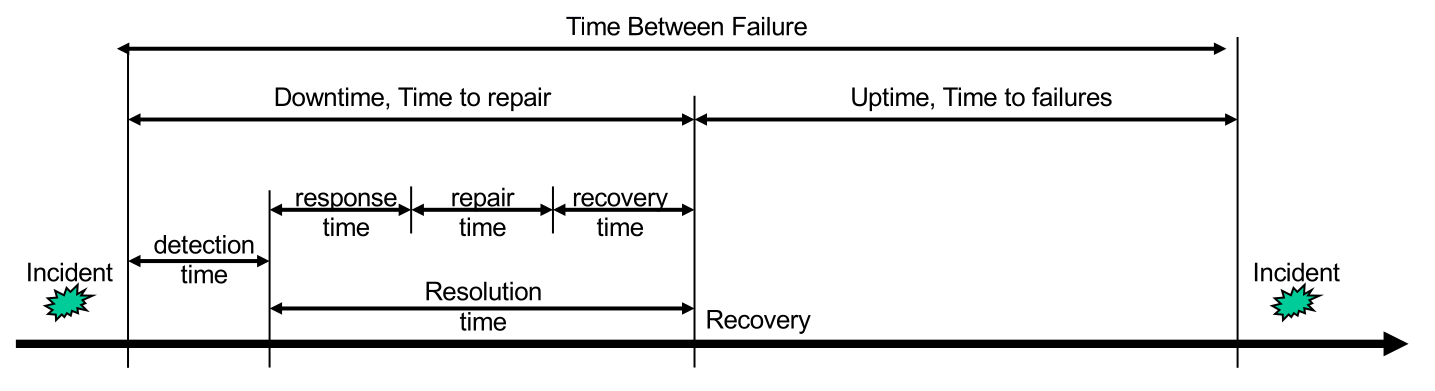
\includegraphics[angle=90, origin=c, width=\linewidth]{6-design/lifecycle-failure.png}
\end{minipage}
\begin{minipage}{0.58\linewidth}
\textbf{Time of occurence}: time at which the user becomes aware of the fault.\\
\textbf{Detection time}: the service provider is informed.\\
\textbf{Response time}: time required by the service provider to respond to the user.\\
\textbf{Repair time}: time required to restore the service or the component that caused the fault.\\
\textbf{Recovery time}: time required to restore the system.\\ \\
\textbf{Mean Time To Repair (MTTR)}: average time between the occurrence of a fault and recovery.\\
\textbf{Mean Time To Failures (MTTF)}: average time between the recovery of an incident and the occurence of the next one.\\
\textbf{Mean Time Between Failures (MTBF)}: average time between the occurrence of two consecutive faults.\\ \\

$MTBF = MTTR + MTTF$.
\end{minipage}

\subsubsection{Availability}
Probability that a component is working properly at a given time.
\[ A = \frac{MTTF}{MTTF + MTTR} \]

Availability in series: $A = \prod A_i$\\
Availability in parallel: $A = 1 - \prod (1 - A_i)$

\subsubsection{Reliability}
Probability that a component has always been working properly during a time interval $(0, t)$.
\[ R = e^{-\lambda t} \qquad \lambda =\frac{1}{MTTF} \]